\documentclass[a4paper,10pt]{article}
\usepackage[pdftex]{graphicx}

% Title Page
\title{Design of the FERS Timing System}
\author{Marc Brooker}


\begin{document}
\maketitle

\begin{abstract}
\end{abstract}

\section{Introduction}
One of the key goals of FERS is to simulate the effects of scheduling of transmissions in networked radar systems. The timing system in FERS intends to model the propagation of timing signals over a network of radars and allow simulation of the effects of timing signals on the performance of such systems.

Another key factor of timing in radar systems is clock jitter and phase noise. The FERS timing system aims to model the effects of jitter on the received radar signal. The timing system does not model the effects of jitter on the sampling process - this modelling is performed seperately on the individual simulated signals.

\section{Structure of a Networked Radar System}
Networked radar systems consist of one or more transmitting stations and one or more receiving stations connected to a central processing and control system. One of the functions of the network is to distribute timing and synchronisation signals to the remote stations, ensuring that they remain synchronised.

\begin{figure}
\centering
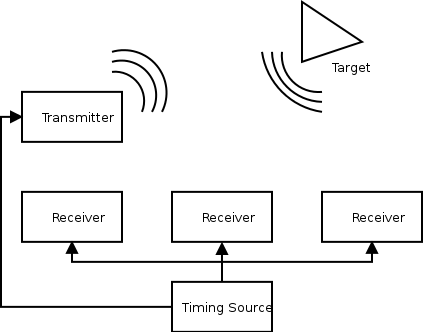
\includegraphics[width=0.8\textwidth]{model}
\caption{Simplified Structure of a Networked Radar System}
\label{fig_block}
\end{figure}

Due to physical constraints, it is not possible to distribute a timing signal in such a way that it arrives at all remote stations simultaneously. The constant difference in time of arrival of synchronisation pulses is trivial to correct if the distance between the stations is known. In addition to this constant difference, the timing signal is also likely to experience both random and deterministic jitter\cite{maxim}.

Figure \ref{fig_block} illustrates a simplified networked radar system. A single timing source connects to all the stations through a network, and the remote stations take their timing from synchronisation pulses produced by the timing source. In order to model the effects of clock propagation through this system, it is necessary to model both the timing source itself and the effects of the network.

\subsection{Timing Source Model}
In FERS, timing sources produce timing pulses with a predetermined frequency. The relative timing of these pulses varies due to the effects of both random and deterministic jitter.

\bibliographystyle{ieeetr}
\bibliography{timing}

\end{document}          
